%%%%%%%%%%%%%%%%%%%%%%%%%%%%%%%%%%%%%%%%%%%%%%%%%%%%%%%%%%%%%%%%%%%%%%%%%%%%
%%%  NiteOutMag --- At Least the Web Remembers What Happened Last Night  %%%
%%%%%%%%%%%%%%%%%%%%%%%%%%%%%%%%%%%%%%%%%%%%%%%%%%%%%%%%%%%%%%%%%%%%%%%%%%%%

\documentclass[runningheads,a4paper]{llncs}

\usepackage[utf8]{inputenc}
\usepackage[T1]{fontenc}
\usepackage[activate=compatibility]{microtype}

% autoref command
%\usepackage[pdftex,urlcolor=black,colorlinks=true,linkcolor=black,citecolor=black]{hyperref}
\def\sectionautorefname{Section}
\def\subsectionautorefname{Subsection}
\def\figureautorefname{Fig.}

\usepackage{graphicx}
\usepackage{xspace}
\newcommand{\googleplus}{Google\nolinebreak\hspace{0em}\raisebox{.28ex}{\tiny\bf +}\kern-0.2ex\xspace}

% listings and Verbatim environment
\usepackage{color}
\usepackage{fancyvrb}
\usepackage{relsize}
\usepackage{listings}
\usepackage{verbatim}
\newcommand{\defaultlistingsize}{\fontsize{8pt}{9.5pt}}
\newcommand{\inlinelistingsize}{\fontsize{8pt}{11pt}}
\newcommand{\smalllistingsize}{\fontsize{7.5pt}{9.5pt}}
\newcommand{\listingsize}{\defaultlistingsize}
\RecustomVerbatimCommand{\Verb}{Verb}{fontsize=\inlinelistingsize}
\RecustomVerbatimEnvironment{Verbatim}{Verbatim}{fontsize=\defaultlistingsize}
\lstset{frame=lines,captionpos=b,numberbychapter=false,escapechar=§,
        aboveskip=0.5em,belowskip=0em,abovecaptionskip=0em,belowcaptionskip=0em,framexbottommargin=-1em,
        basicstyle=\ttfamily\listingsize\selectfont}

\definecolor{lightgray}{rgb}{.9,.9,.9}
\definecolor{darkgray}{rgb}{.4,.4,.4}
\definecolor{purple}{rgb}{0.65, 0.12, 0.82}

\lstdefinelanguage{JavaScript}{
  keywords={typeof, new, true, false, catch, function, return, null, catch, switch, var, if, in, while, do, else, case, break},
  keywordstyle=\color{blue}\bfseries,
  ndkeywords={class, export, boolean, throw, implements, import, this},
  ndkeywordstyle=\color{darkgray}\bfseries,
  identifierstyle=\color{red},
  sensitive=false,
  showstringspaces=false,
  comment=[l]{//},
  morecomment=[s]{/*}{*/},
  commentstyle=\color{purple}\ttfamily,
  stringstyle=\color{black}\ttfamily,
  morestring=[b]',
  morestring=[b]"
}

\hyphenation{NiteOutMag}

\usepackage{comment}
\linespread{0.95}

%%%%%%%%%%%%%%%%%%%%%%%%%%%%%%%
%%%  Beginning of document  %%%
%%%%%%%%%%%%%%%%%%%%%%%%%%%%%%%

\begin{document}

\title{NiteOutMag: At Least the Web\\ Remembers What Happened Last Night}
\titlerunning{NiteOutMag}
\authorrunning{Steiner et al.}

\author{Thomas Steiner\inst{1} \and
		Ruben Verborgh\inst{2} \and
        Rapha\"el Troncy\inst{3} \and\\
		Giuseppe Rizzo\inst{3} \and
		Jos\"e Luis Redondo Garcia\inst{3}		
}

\institute{Universitat Politècnica de Catalunya, Barcelona, Spain\\
  \email{tsteiner@lsi.upc.edu}
  \and
  Ghent University -- IBBT, Belgium\\
  \email{ruben.verborgh@ugent.be}
  \and
  EURECOM, Sophia Antipolis, France\\
  \email{raphael.troncy@eurecom.fr}
}

\maketitle

%%%%%%%%%%%%%%%%%%
%%%  Abstract  %%%
%%%%%%%%%%%%%%%%%%
\begin{abstract}
With NiteOutMag, we present a Chrome Web application that can help people recover what (the hell) happened last night. Among the younger generation, nightlife activities---just about like any other activity---together with related multimedia data get shared online on social networks. The problem is that for one and the same event, the event-related user-generated data may be shared on a plethora of social networks. With this paper, we introduce an application that leverages description of events from several event databases, social data from multiple social networks, and media from some image and video sharing platforms. The data collected is attached to events held in a given area and further processed to generate an event-centric, magazine style presentation, where each page represents an event illustrated by media.
\end{abstract}
\keywords{Event illustration, event reconciliation, media finder, magazine}

%%%%%%%%%%%%%%%%%%%%%%%%%
%%%  1. Introduction  %%%
%%%%%%%%%%%%%%%%%%%%%%%%%

\section{Introduction}                                                      \label{sec:introduction}
In March 2012, 901 million Facebook active users have uploaded more than 300 million photos on average per day\footnote{\url{http://newsroom.fb.com/content/default.aspx?NewsAreaId=22}}. Many of those photos are event-related and typically illustrate events such as music concerts that a user has attended. Facebook, however, is only one among a plethora of social networks that people use to share event-related content. A social network is an online service or media platform that focuses on building and reflecting social relationships among people sharing interests and/or activities. For this paper, we consider eleven different social networks that represent all together most of the Western world's market share. In detail, the considered social networks are
\googleplus (\url{google.com/+}),
Myspace (\url{myspace.com}),
Facebook (\url{facebook.com}),
Twitter ({\url{twitter.com}),
Instagram (\url{instagram.com}),
Flickr (\url{flickr.com}),
YouTube (\url{youtube.com}),
yfrog (\url{yfrog.com}),
MobyPicture (\url{mobypicture.com}),
Twitpic (\url{twitpic.com}), and
\mbox{img.ly} (\url{img.ly}).
Event databases maintain listings of past and upcoming events using crowd sourcing techniques and can be queried programmatically. We include data from four event databases, namely Eventful (\url{eventful.com}), Foursquare (\url{foursquare.com}), Upcoming (\url{upcoming.org}), and Google Places (\url{google.com/places}).

Capturing life moments and building narratives using social networks is addressed in~\cite{Atosy2011}, where the authors investigated about the interaction between event stories and the use of social networks to tell them. They proposed Storify\footnote{\url{http://storify.com/}}, a Web application that supports users to perform story telling. Storyful\footnote{\url{http://storyful.com/}} is an application that allows the user to navigate through stories created by other users or to create new ones, aggregating the content available from Twitter, YouTube, etc. In~\cite{Liu2011}, Liu et al. present a method for combining semantic inferencing and visual analysis for automatically gathering photos and videos illustrating events. With this paper, we propose a way to fully automatically create an event-centric magazine, where each page corresponds to a known event that is illustrated with media shared on the Web. The application\footnote{NiteOutMag application: \url{http://goo.gl/fjuE5}} and a screencast\footnote{Screencast of the NiteOutMag application: \url{https://t.co/3R8h2RnW}} are available.

%%%%%%%%%%%%%%%%%%%%%%%%%%%
%%%  2. Implementation  %%%
%%%%%%%%%%%%%%%%%%%%%%%%%%%

\section{Implementation}                                                    \label{sec:implementation}
The NiteOutMag application is implemented as a Chrome Web application since this technique allows for the whitelisting of specific domains for cross-domain access via \texttt{XMLHttpRequest} calls since not all APIs in use are CORS-enabled.

\paragraph{Geocoding.} The application focuses on events that occurred in a certain area. We use the Google Geocoding API to find the latitude and longitude associated to geographic data, addresses or place names (e.g. \emph{Times Square, New York}).

\paragraph{Event Search.} Based on a latitude and longitude pair, we search for events that took place near the location point in a radius of five kilometers in the recent past using the respective event search APIs. We sanitize the event titles by removing HTML tags, punctuation, common abbreviations (e.g. \emph{w/} for \emph{with} or \emph{ft./feat.} for \emph{featuring}). As event directories can have overlap, we deduplicate events based on the Levenshtein distance of the event titles with an empirically determined editing distance of five. Events descriptions are rdf-ized and reconciled as performed in EventMedia~\cite{Khrouf2012}.

\paragraph{Media Search.} Unlike event search, media search in our application is \emph{not} based on geolocation. Seline reports in May 2012 that only 1\% of all microposts on Twitter are geotagged\footnote{\url{http://www.quora.com/What-percentage-of-Twitter-photos-are-geotagged}} and not all social networks support geotagging of content. Consequently, we use a two-tier approach for media search: We define as \emph{human-friendly address} the first part up to the comma of the \texttt{formatted\_address} field in the Google Geocoding API. We perform then a full-text search for:
\begin{itemize}
 \item \emph{(i)} the (event name) $+$ the (venue name) and
 \item \emph{(ii)} the (event name) $+$ the (human-friendly address).
\end{itemize}
We have implemented a media collector consisting of media extractors for all social networks listed in Section~\ref{sec:introduction}. It takes a search term as an input (\emph{e.g.} \emph{Beach Boys Columbia}) and then performs a parallel full-text search using the search APIs of the social networks. When all the media extractors have responded, a unified output is delivered. We propose a common alignment schema, illustrated in Listing~\ref{lst:media} which shows the resulting metadata for an exemplary media item. Figure~\ref{fig:architecture} depicts the overall architecture of the media collector.
\begin{lstlisting}[language=JavaScript,caption={Sample output of the media collector showing a Google+ post},label={lst:media}]
{
  "mediaurl": "http://t.co/ubagkiR9",
  "storyurl": "https://t.co/dau5pBWD",
  "message": {
    "text": "My wife, who once said her vision of
        heaven was being on the lawn bouncing
        around beach balls at a Beach Boys
        concert [...]
        <a href=\"http://t.co/pH2OV1fW\" >
        http://t.co/pH2OV1fW</a> [...]",
    "clean": "My wife, who once said her vision of
        heaven was being on the lawn bouncing
        around beach balls at a Beach Boys
        concert [...]"
  },
  "user": "https://t.co/gIf2UVZR",
  "type": "photo",
  "timestamp": 1329342797000,
  "published": "2012-02-15T21:53:17.000Z"
}
\end{lstlisting}

\paragraph{Magazine Layout.} In order to create the illusion of a real magazine, the ability of flipping from page to page needs to be as credible as possible. The open-source library \texttt{turn.js} by Emmanuel García~\footnote{\texttt{turn.js} library (\url{http://www.turnjs.com/})} allows for the dynamic creation of magazines solely based on HTML5 technologies with a very realistic page flip effect. We treat each event as one page of the magazine, add the event metadata as headline and subheading of the page, and arrange the images and accompanying microposts to fill up the page. For each event, we use the image with the highest resolution as background image of the page in order to create a lifestyle magazine appearance. For additional print-like look and feel, we use drop caps (Figure~\ref{fig:screenshot}). The title page gets dynamically created based on a Google image search for the (human-friendly address) $+$ the keyword (nightlife).
\begin{figure*}[htb!]
\centering
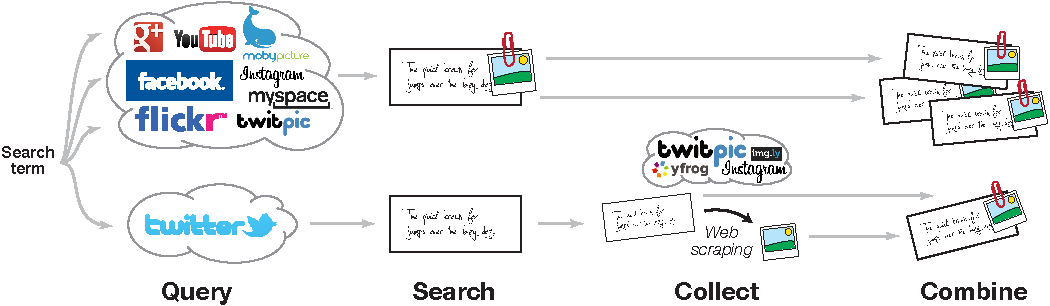
\includegraphics[width=0.6\linewidth]{./architecture.pdf}
\caption{Overview of the media collector: hybrid approach for the media item extraction process using a combination of API access and Web scraping}
\label{fig:architecture}
\end{figure*}
\begin{figure}[htbp]
\centering
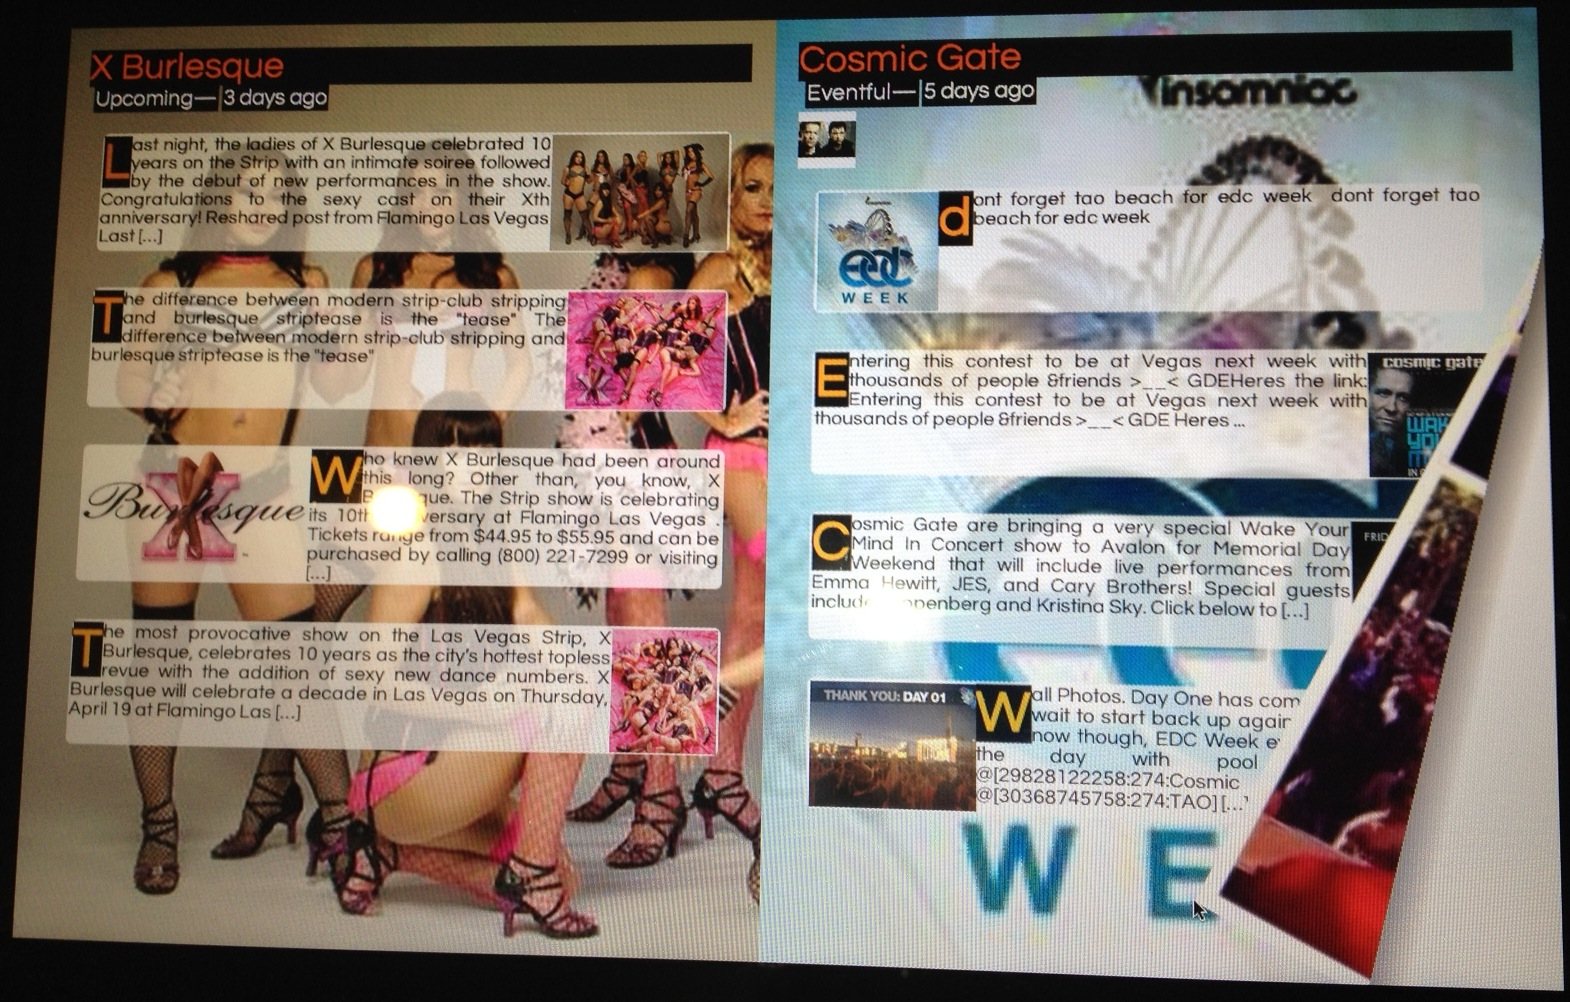
\includegraphics[width=1.0\columnwidth]{./screenshot.jpg}
\caption{Screenshot of the NiteOutMag application with two events from Las Vegas and the righthand-side page about to be flipped}
\label{fig:screenshot}
\end{figure}

%%%%%%%%%%%%%%%%%%%%%%%
%%%  3. Conclusion  %%%
%%%%%%%%%%%%%%%%%%%%%%%

\section{Conclusion}
%The results stand and fall with the quality of the events in the event databases. One of the problems we encountered are event titles such as
%\emph{Kandyland 2012 @ the Playboy Mansion -- 1.877.VIP.MANSION}\footnote{Kandyland 2012 event (\url{http://t.co/YUm7FtmE})}, which combine the event name with the venue name and a~vanity contact phone number. The detection of such composed titles is difficult and requires advanced linguistic processing. Event deduplication is a second issue. The two movie events \emph{The Avengers} and \emph{Marvel's The Avengers 3D} are the same for a human being. However, for a machine, the duplication is harder to detect. Media item deduplication is a task that we have left for future work.

We have presented a Chrome Web application that illustrates events via four event databases and eleven social networks and media sharing platforms. Semantic web technologies are used all along the way for integrating and reconciling those heterogenous sources. The application harvests event-related data on-the-fly for a user-determined center of interest and compiles the data in an aesthetic lifestyle magazine. Using popular party destinations, big cities, and places of interests, we have evaluated the retrieved results for both relevancy and visual appeal, with a~special focus on optimized recall. While there are actionable issues for future work, we are quite happy with the outcome so far.

%%%%%%%%%%%%%%%%%%%%%%%%%
%%%  Acknowledgments  %%%
%%%%%%%%%%%%%%%%%%%%%%%%%

%\section*{Acknowledgments}                                                   \label{sec:acknowledgments}
%T. Steiner is partially supported by the European Commission under Grant No.~248296 FP7 (\mbox{I-SEARCH} project). R. Verborgh is funded by Ghent University,
%the Interdisciplinary Institute for Broadband Technology~(\mbox{IBBT}), the Institute for the Promotion of Innovation by Science and Technology in Flanders~(\mbox{IWT}), the Fund for Scientific Research Flanders~(\mbox{FWO} Flanders), and the European Union. R. Troncy is partially supported by the French National Agency under contracts ANR.11.EITS.006.01, ``Open Innovation Platform for Semantic Media'' (OpenSEM) and the European Union's 7$^{th}$ Framework Programme via the project LinkedTV (GA 287911).

%%%%%%%%%%%%%%%%%%%%%%
%%%  Bibliography  %%%
%%%%%%%%%%%%%%%%%%%%%%

\bibliographystyle{abbrv}
\bibliography{iswc2012}

\end{document}
